\documentclass[sigplan,review,anonymous,nonacm]{acmart}\settopmatter{printfolios=true,printccs=false,printacmref=false}



\setcopyright{none}

\usepackage{minted}

\bibliographystyle{ACM-Reference-Format}
%% Some recommended packages.
\usepackage{booktabs}   %% For formal tables:
                        %% http://ctan.org/pkg/booktabs
\usepackage{subcaption} %% For complex figures with subfigures/subcaptions
                        %% http://ctan.org/pkg/subcaption



\newcommand\question[1]{{\color{violet}#1}}
\newcommand\todo[1]{{\color{red}#1}}

\begin{document}



\title{Hardware and software co-design for sparse linear algebra operations acceleration} 


\maketitle

\section{Scope of problem}
Matrices and the corresponding operations are well-established components for data representation and analysis since it allows to tackle a problem with the help of a myriad of matrix accelerators. However, the data is inherently sparse in many modern applications, e.g., social graphs have far less edges than vertices~\cite{leskovec2016snap}. Such a high sparsity incurs both computational and storage inefficiencies, requiring an unnecessarily large storage, occupied by zero elements, and a large number of operations on zeroes, where the result is obviously known beforehand. The traditional approach to address these inefficiencies is to compress the
matrix and store only the non-zero elements, and then operate only
on the non-zero values.
Thus, the effect of matrices tending to be sparse in many applications makes the techniques of matrix compressed representation and sparse linear algebra to be the effective way of tackling problems in areas including but not limited to graph analysis~\cite{GAILLA}, computational biology~\cite{compBio} and machine learning~\cite{Kepner_2017}.

Sparse linear algebra defines building blocks for expressing algorithms for mentioned areas in a uniform way in terms of sparse matrix and vector operations over some semiring. Once such blocks are implemented in software (or hardware) according to, e.g., \emph{GraphBLAS}~\cite{buluc2017graphblas} standard, a plenty of expressible algorithms could be tuned and optimized at once by optimizing and tuning the building blocks. One of the key primitives is a sparse matrix-sparse matrix multiplication (spMspM) operation. It has high-performance implementations both for CPUs and GPUs. However, typical CPUs and GPUs are proven to be underutilized~\cite{Florida,leskovec2016snap,Song_2016,zhang2020sparch}, i.e., their computing units do not achieve peak performance, for tasks that involve sparsity, due to being too general by design and suffering from the irregularity of memory accesses incurred by sparsity. Further, the pipeline of spMspM is patchy, which makes some of the computational units to be idle from time to time as it could be seen in~\ref{fig:sm_util}, while the peak FLOPS is less than 1\% of maximum available.

\footnotetext{\url{https://developer.nvidia.com/cusparse} (Accessed 09.02.2021)}


To address this issue several specialized hardware accelerators have been designed for spMspM~\cite{OuterSpace,zhang2020sparch}. However, for a sparse framework to be useful, it should incorporate not only spMspM, but also other sparse operations parameterized by a semiring, e.g., masking, which filters the matrix elements or element-wise operations needed for, e.g., PageRank and bread-first search (BFS) algorithms~\cite{yang2020graphblast}. And when such operations are chained explicitly or implicitly, via a loop body, certain optimizations could be applied. However, some of such optimizations are only expressible at software level, i.e., in programming language, thus modern spMspM accelerators could be impractical for accelerating the whole program representing a linear algebra based algorithm like PageRank or BFS, due to the lack of a software part and to a too narrow hardware specialization. Thus a co-design of dedicated hardware and software components, i.e., domain-specific processor (DSP) and a corresponding domain-specific language (DSL), could provide a system which is not more effective for spMspM than present hardware accelerators, but appear to be more effective in terms of speed and power consumption for holistic pieces of program, i.e., for chained operations, than current CPUs and GPUs implementations. The ongoing work is devoted to the design of respective DSL, DSP, and an optimizing compiler, and this work in particular discusses the ideas and challenges behind the design. 



% \begin{listing}[t]
% \caption{Breadth-first search example}
% \label{listing:1}
% \begin{center}

% \begin{minted}{python}
% #Sparse algebra BFS:
% #times: if (A[i,j] != 0) A[i,j] × q(k) = k
% #       else 0
% #plus : any(x,y) = x or y randomly

% q = [source]; 
% parent = [0 for i in range(n)]; 
% parent[source] = source;

% while (q not empty)
%     #masked matrix vector multiplication
%     q<¬parent> = A*q #mask could be inverted
%     #masked assignment
%     parent<q> = q
% \end{minted}
    
% \end{center}
% \end{listing}

\begin{figure}[t]
    \centering
    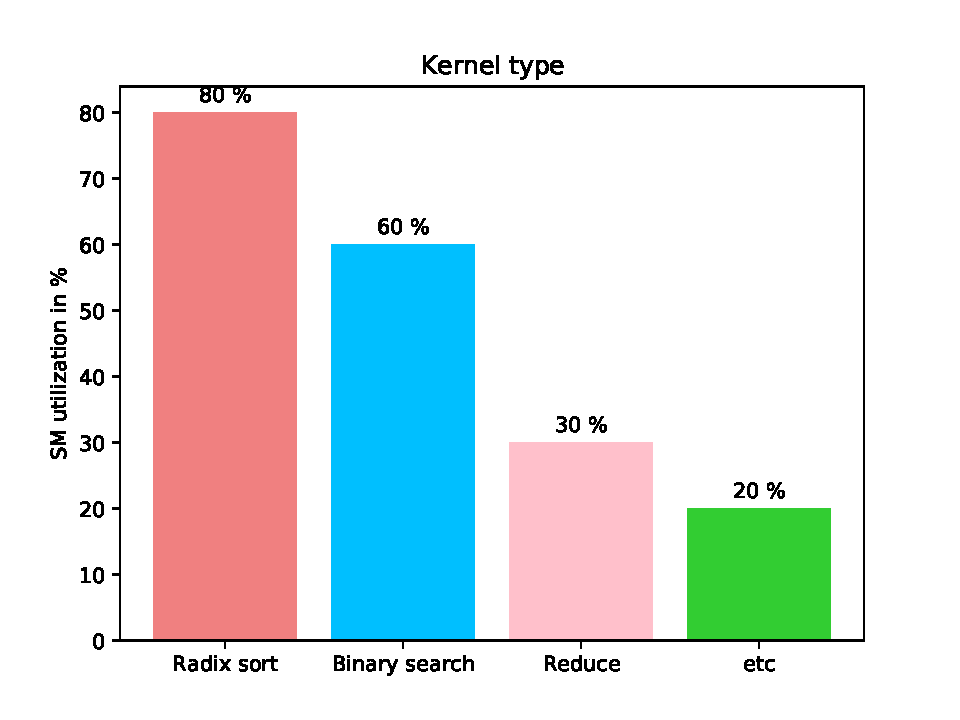
\includegraphics[width=\linewidth]{figures/SM_perforance.pdf}
    \caption[Caption for LOF]{GPU's SM utilization for spMspM pipeline from cuSPARSE\footnotemark}
    \label{fig:sm_util}
\end{figure}

\section{Optimizations}

Since sparse linear algebra applications are mostly concerned with graph problems, some of the optimizations are graph-specific~\cite{yang2020graphblast,graphIt}, e.g., direction optimization. In this work, we are mostly interested in graph-agnostic optimizations, where the most considered~\cite{yang2020graphblast,graphIt} one is \emph{fusion}~\cite{fusion}, which in essence stands for deleting intermediate data structures merging several operations into one along the way. 

The problem of intermediate data structures is common for functional programming and there have been developed a number of optimization techniques that try reduce intermediate data structures or computations, namely partial evaluation~\cite{jones}, deforestation~\cite{WADLER1990231}, supercompilation~\cite{supercompilation}, and distillation~\cite{distillation}. All of these optimization will be reffered as fusion futher. The purpose of such optimizations is to remove intermediate structures, e.g., lists, in scenarios like

\begin{minted}[escapeinside=//]{haskell}
f :: Int /$\rightarrow$/ Int
f n = sum [ k * m | k /$\leftarrow$/ [1..n], m /$\leftarrow$/ [1..k] ] 
\end{minted}

or optimize recursive calls like

\begin{minted}[escapeinside=//]{haskell}
nrev :: [a] /$\rightarrow$/ [a]
nrev [] = []
nrev x:xs = app (nrev xs) [x]

app :: [a] /$\rightarrow$/ [a]
app [] xs = xs
app (x:xs) ys = x : app xs ys

-- optimizing quadratic nrev to
arev xs = arev' xs []
arev' [] ys = ys
arev' (x:xs) ys = arev' xs (x : ys)
\end{minted}

For the case of sparse linear algebra such optimizations are expected to fuse operations removing intermediate matrices, e.g. eliminating \texttt{A ewiseAdd B} matrix in

\begin{minted}{haskell}
D = A ewiseAdd B ewiseMult C
\end{minted}
 
 or fusing a mask with sparse matrix-vector multiplication reducing the number of memory accesses~\cite{yang2020graphblast}.
 
 These fusion family optimizations are implementation dependent, meaning that the optimizer should have an access to the source code, which is impossible when the function is implemented solely in hardware. However, arbitrary functions could be fused using rules like 
\begin{minted}[escapeinside=||]{haskell}
 map f (map g ls) |$\equiv$| map (f |$\circ$| g) ls 
\end{minted}
where the $\circ$ is function composition, but this would require a specialized hardware unit for each function which is impractical. Further, such optimizers produce a code that essentially represents a dataflow through constructors / destructors and corresponding semiring operations, which seems to fit dataflow processor architecture. Thus we believe that a functional DSL, where an arbitrary semiring could be concisely and conveniently expressed, powered by a set of optimizers and compilable to some dataflow DSP with enough parallelism could be a good starting point in acceleration of sparse linear algebra based programs. However there are several challenges present, some of which are incurred by the implementation-dependent nature of the optimizers. 
% In case of sparse linear algebra operations, fusion is able, e.g., to fuse masking with sparse matrix-vector multiplication, eliminating intermediate matrix and reducing the number of memory accesses~\cite{yang2020graphblast} or to fuse a chain of element-wise operations into one. However, the implementation-dependent nature of fusion incurs some challenges.

\section{Challenges}
Firstly, not every operation could be fused, e.g., sorting, which is a noticeable part of sparse pipeline~\ref{fig:sm_util} or union / intersection, making it reasonable to implement such operations solely in hardware. Every such operation should be identified and implemented as a processing element inside the processor under design. However, the need for such operations depends on the particular compressed representation of a matrix, which strongly affects the pattern of memory accesses and henceforth the dataflow and the overall performance, e.g. compressed-row format requires sorting while quad-tree~\cite{qtree} representation does not. 

Secondly, the matrix compression format affects the amena\-bility for optimizations. There are many techniques for list and stream fusion~\cite{StreamFusion,StreamFusion2}, but such data structures are not effective for irregular indexing accesses incurred by a particular compressed representation, e.g., compressed-row format. Conversely, the representation that does not incur many such accesses could be fused successfully with the known techniques but cannot be processed in parallel so well. The state-of-the-art fusion systems on top of arrays, which are effective for random accesses, presently are not smart enough to fuse something with index arithmetic~\cite{Futhark}. Once again quad-tree representation seems to be amenable for fusion and parallelization.

Thirdly, to achieve the full benefit from fusion, the key primitives should be implemented with fusion in mind, which is not trivial and again depends on the compressed representation of choice.

% Fourthly, the benefit from fusion differs in cases when the memory could be allocated dynamically effectively and not, e.g., in case of GPUs most implementations of spMspM precompute the size of the resulting matrix with another kernel allocation inside a kernel is 
Finally, the main challenge is to choose a processor architecture which would allow it to execute the fused programs most effectively. For example, the result of some of the optimizations perform poor on SIMD devices like GPUs, due to, e.g., thread divergence. Hence, the processor architecture seems to should be MIMD one and should be general enough to support arbitrary semirings and specialized enough to be effectively utilized. One prominent architecture is Transport Triggered Architecture (TTA)~\cite{TCEToolset}, which is simple and inherently parallel~\cite{FPTTA}.


\section{Evaluation}
At the moment we focus on exploiting a supercompiler \question{distillator?} to perform a fusion for a subset of GraphBLAS operations, using a quad-tree representation and aim to target TTA architecture. If the approach is successful it is supposed to be compared with state-of-the-art CPUs and GPUs implementations of GraphBLAS standard~\cite{SuiteSparse,yang2020graphblast}
first in simulation and then on an FPGA board. Otherwise we will explore other compressed matrix representations and / or extend the optimizers if possible.

% \begin{listing}
% \centering
% \caption{Fusion for the composition of \texttt{append} functions}
% \label{listing:fusion}
% \begin{minted}{haskell}
% app [] ls = ls
% app (x:xs) ls = x : app xs ls

% -- call for this function

% app (app xs ys) zs

% -- is fused to the following function definition
% -- that is specialized for three lists

% f [] xs ys = g xs ys
% f (x:xs) ys zs = x : f xs ys zs

% g [] xs = xs
% g x:xs ys = x : g xs ys

% -- and a call
% f xs zs ys

% \end{minted}

% \end{listing}



\bibliography{bib}
\end{document}
